\documentclass{beamer}
\usepackage{amsmath,amssymb,latexsym,array,fancyheadings,mathdots}
\usepackage{algorithm,algorithmic}
\usepackage{hyperref}
\usepackage{color}
\usepackage{tabularx}
\usepackage[all]{xy}
\usepackage{qtree}
\usepackage{gitinfo2}

%% RCS
%\usepackage{rcs}

%% Colors
\definecolor{darkgreen}{rgb}{0,.4,0}
\definecolor{darkred}{rgb}{.5,0,0}
\definecolor{darkmagenta}{rgb}{.5,0,.5}
\definecolor{orange}{rgb}{1,.5,0}
\definecolor{lightblue}{rgb}{0.122,0.016,0.855}
\definecolor{darkocre}{rgb}{0.471,0.298,0.008}

\usetheme{default}

%% New Theorems
\newtheorem{thm}{Theorem}
\newtheorem{exm}[thm]{Example}
\newtheorem{cor}[thm]{Corollary}
\newtheorem{propo}[thm]{Proposition}
\newtheorem{lem}[thm]{Lemma}
\newtheorem{clm}[thm]{Claim}
\newtheorem{exr}[thm]{Exercise}
\newtheorem{dfn}[thm]{Definition}

%% New commands
\newcommand{\classfont}{\mathsf}
\newcommand{\ATM}{\classfont{A}_{\mathrm{TM}}}
\newcommand{\MTF}{\mathrm{MTF}}
\newcommand{\OPT}{\mathrm{OPT}}
\newcommand{\ALG}{\mathrm{ALG}}
\newcommand{\ALGNAIVE}{\mathrm{ALG}_{\text{na{\"\i}ve}}}
\newcommand{\LRU}{\mathrm{LRU}}
\newcommand{\FIFO}{\mathrm{FIFO}}
\newcommand{\FWF}{\mathrm{FWF}}
\newcommand{\LFD}{\mathrm{LFD}}
\newcommand{\true}{\mathsf{T}}
\newcommand{\false}{\mathsf{F}}
\newcommand{\also}{\wedge}
\newcommand{\lra}{\leftrightarrow}
\newcommand{\tc}{\textcolor}
\newcommand{\df}[1]{\textcolor{red}{\em #1}}
\newcommand{\highlight}[1]{\textcolor{orange}{\em #1}}
\newcommand{\hl}[1]{\textcolor{blue}{\em #1}}
\newcommand{\amp}{\texttt{\&}}
\newcommand{\hsh}{\texttt{\#}}
\newcommand{\ra}{\rightarrow}
\newcommand{\longra}{\longrightarrow}
\newcommand{\Ra}{\Rightarrow}
\newcommand{\rab}{{\rightarrow_\beta}}
\newcommand{\srab}{{\rightarrow^*_\beta}}
\newcommand{\aeq}{{=_\alpha}}
\newcommand{\order}{\mathrm{order}}
\newcommand{\rem}{\mathrm{rem}}
\newcommand{\IP}{\mathbf{IP}}
\newcommand{\PSPACE}{\mathbf{PSPACE}}
\newcommand{\thevalue}{\text{value}}
\newcommand{\pol}[1]{\mathbf{#1}}
\newcommand{\enc}{\text{Enc}}
\newcommand{\xor}{\oplus}
\newcommand{\zo}{\{0,1\}}
\newcommand{\SOPT}{S_{\mathrm{opt}}}
\newcommand{\la}{\leftarrow}
\newcommand{\myurl}[1]{\textcolor{darkgreen}{\url{#1}}}
\newcommand{\myhref}[2]{\textcolor{darkgreen}{\href{#1}{#2}}}
\newcommand{\qaccept}{q_{\mathrm{accept}}}
\newcommand{\qreject}{q_{\mathrm{reject}}}
\newcommand{\opt}{\text{\sc Opt}}
\newcommand{\tr}{\mathrm{tr}}
\newcommand{\csanky}{p^{\textsc{csanky}}}
\newcommand{\berk}{p^{\textsc{berk}}}

%% Algorithms package customization
\renewcommand{\algorithmicrequire}{\textbf{Pre-condition:}} 
\renewcommand{\algorithmicensure}{\textbf{Post-condition:}} 
\algsetup{indent=3em}

\input{prooftree}

%% including/excluding pauses
\newcommand{\ifpause}{\iftrue} % for including pauses
%\newcommand{\ifpause}{\iffalse} % for excluding pauses

%% 2nd or 3rd edition
\newif\ifthird
\thirdtrue
%\thirdfalse

%disables usefoottemplate
\setbeamertemplate{navigation symbols}{}
%\setbeamertemplate{footline}% 
%{\strut\quad\tiny 
%\begin{minipage}{3cm}
%Cryptography - Michael Soltys
%\today\ {\tt v\RCSRevision}
%\end{minipage}\hfill
%\insertsection\
%- \insertframenumber/\inserttotalframenumber\quad\strut}

\newcommand{\mytitle}{Randomized}
\newcommand{\mychpnr}{6}
%% Title page contents
\title{Intro to Analysis of Algorithms \\ \mytitle \\  Chapter \mychpnr}
\author{Michael Soltys}
\date{\textcolor{darkgreen}{\tiny\tt 
[ {\bf Git} Date:\gitAuthorDate\ 
Hash:\gitAbbrevHash\ 
Ed:\ifthird
3rd
\else
2nd
\fi]}}
\institute{CSU Channel Islands}

\setbeamertemplate{footline}{
  \colorbox{white}{\color{black}\tt
     \begin{tabularx}{0.97\textwidth}{XXX}
          IAA Chp \mychpnr\ - Michael Soltys \copyright & 
          \hfill\today\ (\gitAbbrevHash; \ifthird ed3\else ed2\fi)
					\hfill\phantom{.} & 
          \hfill\insertsection\ - \insertframenumber/\inserttotalframenumber \\
      \end{tabularx}}}

\begin{document}

\mode<presentation>
{
}

\parskip 8pt

\section{Introduction}

\begin{frame}
\titlepage
\end{frame}


\section{Introduction}

%\addfootbox{\tiny}

\section{Primality testing}

\begin{frame}
\frametitle{Primality testing}

One way to determine whether a number $p$ is prime, is to try all
possible numbers $n<p$, and check if any are divisors.

This brute force procedure has exponential time complexity
in the length of $p$, and so it has a prohibitive time cost.  
\end{frame}

\begin{frame}
{Sieve of Eratosthenes}

\begin{minipage}{2cm}
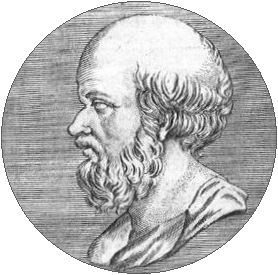
\includegraphics[width=2cm]{Figures/Eratosthene.png}
\end{minipage}
\begin{minipage}{6cm}
Eratosthenes of Cyrene \\
Born $\sim 276$ BC and died $\sim 194$ BC \\
Chief librarian at Library of Alexandria
\end{minipage}

Algorithm for finding all primes $\le n$.
\begin{algorithmic}[1] 
  \STATE  $L=\{2,3,4,\ldots,n\}$
  \STATE  $p=2$
	\STATE  Mark all $2p,3p,4p,\ldots$ on list $L$ 
	\STATE  Find first unmarked number greater than $p$, say $k$.
	\STATE  Repeat with $p=k$
\end{algorithmic}

See simulation here:
\url{https://en.wikipedia.org/wiki/Sieve_of_Eratosthenes}
\end{frame}

\begin{frame}
Although a polytime (deterministic) algorithm for primality is now
known\footnote{Agrawal, Kayal and Saxena, August 2002.}, the
Rabin-Miller \highlight{randomized algorithm} 
for primality testing is simpler and
more efficient, and therefore still used in practice.
\end{frame}

\begin{frame}
Testing primality with {\tt openssl version}: 
\begin{quote}
OpenSSL 1.0.2g  1 Mar 2016
\end{quote}

{\tt openssl prime 348911131111712333333111111111}
\end{frame}

\begin{frame}
Fermat's Little theorem
provides a ``test'' of sorts for primality,
called the Fermat test; the Rabin-Miller algorithm
is based on this test.  When we say
that $p$ passes the Fermat test at $a$, what we mean is that
$a^{(p-1)}\equiv 1\pmod p$.  Thus, all primes pass the Fermat test for
all $a\in\mathbb{Z}_p-\{0\}$.  

Unfortunately, there are also composite numbers $n$ that pass the
Fermat tests for every $a\in\mathbb{Z}_n^*$; these are the so called
{\em Carmichael numbers}, for example, 561, 1105, 1729, etc.
\end{frame}

\begin{frame}
If $p$ is a composite non-Carmichael number, then it passes at most
half of the tests in $\mathbb{Z}_p^*$.  That is, if $p$ is a composite
non-Carmichael number, then for at most half of the $a$'s in the set
$\mathbb{Z}_p^*$ it is the case that $a^{(p-1)}\equiv 1\pmod p$.

Call $a$ a {\em witness} (for $p$) if it fails the Fermat test for
$p$, that is, $a$ is a witness if $a^{(p-1)}\not\equiv 1\pmod p$.  Let
$S\subseteq\mathbb{Z}_p^*$ consist of those elements
$a\in\mathbb{Z}_p^*$ for which $a^{p-1}\equiv 1\pmod p$.  It is easy
to check that $S$ is in fact a subgroup of $\mathbb{Z}_p^*$.

Therefore, by Lagrange theorem
$|S|$ must divide $|\mathbb{Z}_p^*|$.  Suppose now that there exists
an element $a\in\mathbb{Z}_p^*$ for which $a^{p-1}\not\equiv 1\pmod
p$.  Then, $S\neq\mathbb{Z}_p^*$, so
the next best thing it can be is ``half'' of $\mathbb{Z}_p^*$, so
$|S|$ must be at most half of $|\mathbb{Z}_p^*|$.  
\end{frame}

\begin{frame}
A number is {\em pseudoprime} if it is either prime or Carmichael.

The last result suggests an algorithm for pseudoprimes: on input $p$,
check whether $a^{(p-1)}\equiv 1\pmod p$ for some random
$a\in\mathbb{Z}_p-\{0\}$.  

If $p$ fails this test (i.e.,
$a^{(p-1)}\not\equiv 1\pmod p$), then $p$ is composite for sure.  

If
$p$ passes the test, then $p$ is probably pseudoprime.  

We show that
the probability of error in this case is $\le\frac{1}{2}$.  

Suppose
$p$ is not pseudoprime.  If $\gcd(a,p)\neq 1$, then
$a^{(p-1)}\not\equiv 1\pmod p$, so assuming that $p$ passed the test,
it must be the case that $\gcd(a,p)=1$, and so $a\in\mathbb{Z}_p^*$.
But then at least half of the elements
of $\mathbb{Z}_p^*$ are witnesses of non-pseudoprimeness.
\end{frame}

\begin{frame}
Show that if $\gcd(a,p)\neq 1$ then $a^{(p-1)}\not\equiv 1\pmod p$.

The informal algorithm for pseudoprimeness described in the paragraph
above is the basis for the Rabin-Miller algorithm which we discuss
next.  The Rabin-Miller algorithm extends the pseudoprimeness test to
deal with Carmichael numbers.

\end{frame}

\begin{frame}
\frametitle{Rabin-Miller algorithm}

\begin{algorithmic}[1] 
   \STATE  If $n=2$, accept; if $n$ is even and $n>2$, reject. 
   \STATE  Choose at random a positive $a$ in $\mathbb{Z}_n$. 
   \IF {$a^{(n-1)}\not\equiv 1\pmod n$} 
       \STATE reject
   \ELSE 
            \STATE Find $s,h$ such that $s$ is odd and $n-1=s2^h$
            \STATE Compute the sequence
                $a^{s\cdot 2^0},a^{s\cdot 2^1},a^{s\cdot 2^2},
                 \ldots,a^{s\cdot 2^h}\pmod n$
      \IF{all elements in the sequence are~1} 
            \STATE accept
      \ELSIF{the last element different from~1 is $-1$} 
            \STATE accept
      \ELSE 
            \STATE reject
      \ENDIF
    \ENDIF
\end{algorithmic}

\end{frame}

\begin{frame}

Note that this is a polytime (randomized) algorithm.

If $n$ is a prime then the Rabin-Miller algorithm accepts it; if $n$
is composite, then the algorithm rejects it with probability
$\ge\frac{1}{2}$.

If $n$ is prime, then by Fermat's Little 
theorem $a^{(n-1)}\equiv 1\pmod n$,
so line~4 cannot reject $n$.  Suppose that line~13 rejects $n$; then
there exists a $b$ in $\mathbb{Z}_n$ such that $b\not\equiv\pm
1\pmod n$ and $b^2\equiv 1\pmod n$.  Therefore, $b^2-1\equiv 0\pmod
n$, and hence
$$
(b-1)(b+1)\equiv 0\pmod n.
$$
Since $b\not\equiv\pm 1\pmod n$, both $(b-1)$ and $(b+1)$ are strictly
between $0$ and $n$, and so a prime $n$ cannot divide their product.
This gives a contradiction, and therefore no such $b$ exists, and so
line~13 cannot reject $n$.

\end{frame}

\begin{frame}

If $n$ is an odd composite number, then we say that $a$ is a
\df{witness} (of compositness) for $n$ if the algorithm rejects on
$a$.

We show that if $n$ is an odd composite number, then at least half of
the $a$'s in $\mathbb{Z}_n$ are witnesses.  

The distribution of
witnesses in $\mathbb{Z}_n$ appears to be very irregular, but if we
choose our $a$ ``uniformly at random,'' we hit a witness with probability
$\ge\frac{1}{2}$.

Because $n$ is composite, either $n$ is the power of an odd prime, or
$n$ is the product of two odd co-prime numbers.

This yields two cases.

\end{frame}

\begin{frame}

{\bf Case 1.}  Suppose that $n=q^e$ where $q$ is an odd prime and
$e>1$.  

\begin{equation}\label{eq:firstt}
\text{Set } t:=1+q^{e-1}
\end{equation}

From the binomial expansion of $t^n$ we
obtain:
\begin{equation}\label{eq:witness}
t^n=(1+q^{e-1})^n=1+nq^{e-1}+\sum_{l=2}^n\binom{n}{l}(q^{e-1})^l,
\end{equation} 

\begin{equation}\label{eq:secondt}
\therefore t^n\equiv 1\pmod n
\end{equation}

\end{frame}

\begin{frame}

\begin{itemize}
\item  If $t^{n-1}\equiv 1\pmod n$,
then $t^n\equiv t\pmod n$ which contradicts~(\ref{eq:firstt})
and~(\ref{eq:secondt}).  

Hence $t$ is a line~4 witness.  

\item  But the set of
line~4 non-witnesses, 
$$
S_1:=\{a\in\mathbb{Z}_n|a^{(n-1)}\equiv 1\pmod n\},
$$
is a \highlight{\em proper} subgroup of $\mathbb{Z}_n^*$

Note that $t\in\mathbb{Z}^*-S_1$

by Lagrange's theorem $S_1$ is at
most half of $\mathbb{Z}_n^*$, and so it is at most half of
$\mathbb{Z}_n$.
\end{itemize}

\end{frame}

\begin{frame}

{\bf Case 2.}  Suppose that $n=qr$, where $q,r$ are co-prime.

Among all line~13 non-witnesses, find a non-witness for which the
$-1$ appears in the largest position in the sequence in line~7 of the
algorithm 

Note that $-1$ is a line~13 non-witness, so the set of these
non-witnesses is not empty.  

Let $x$ be such
a non-witness and let $j$ be the position of $-1$ in its sequence,
where the positions are numbered starting at 0;  $x^{s\cdot
2^j}\equiv -1\pmod n$ and $x^{s\cdot 2^{j+1}}\equiv 1\pmod n$.  

The
line~13
non-witnesses are a subset of 
$$
S_2:=\{a\in\mathbb{Z}_n^*|a^{s\cdot 2^j}\equiv\pm 1\pmod n\},
$$
and $S_2$ is a subgroup of
$\mathbb{Z}_n^*$.

\end{frame}

\begin{frame}

By the CRT there exists $t\in\mathbb{Z}_n$ such that
$$
\begin{array}{l}
t\equiv x\pmod q \\
t\equiv 1\pmod r
\end{array}
\quad\Rightarrow\quad
\begin{array}{l}
t^{s\cdot 2^j}\equiv -1\pmod q \\
t^{s\cdot 2^j}\equiv 1\pmod r
\end{array}
$$
Hence $t$ is a witness because $t^{s\cdot 2^j}\not\equiv\pm 1\pmod
n$  but on the other hand $t^{s\cdot 2^{j+1}}\equiv 1\pmod n$.  

Exercise: Show that $t^{s\cdot 2^j}\not\equiv\pm 1\pmod n$.

Therefore, just as in case~1, we have constructed a
$t\in\mathbb{Z}_n^*$ which is not in $S_2$, and so $S_2$ can be at
most half of $\mathbb{Z}_n^*$, and so at least half of the elements in
$\mathbb{Z}_n$ are witnesses.
\end{frame}

\begin{frame}
Note that by running the algorithm $k$ times on independently chosen
$a$, we can make sure that it rejects a composite with probability
$\ge 1-\frac{1}{2^k}$ (it will always accept a prime with
probability~1).  

Thus, for $k=100$ the probability of error, i.e., of
a false positive, is \highlight{negligible}.
\end{frame}

\begin{frame}
{Summarize 3 important points}

\begin{enumerate}
\item  Rabin-Miller has 50\%\ of a false-positive, but we can
\highlight{amplify it away} by repeating the test to
\highlight{negligable}.

\item  As there are lots of primes ($\pi(n)\rightarrow n/\log(n)$) we
can convert easily a tester of primes into a \highlight{generator of
primes}.

\item  For implementation we still have to show how to compute
$$
g^x\pmod n
$$ 
for large $x$, say in the order of 4K bits:
\highlight{repeated squaring trick}. 
\end{enumerate}
\end{frame}

\begin{frame}
{Repeated Squaring}

Computing large powers in $(\mathbb{Z}_n,\ast)$ can be done
efficiently with \df{repeated squaring}---for example, if
$(m)_b=c_r\ldots c_1c_0$, then compute
$$
a_0=a,a_1=a_0^2,a_2=a_1^2,\ldots, a_r=a_{r-1}^2\pmod n,
$$
and so $a^{m}=a_0^{c_0}a_1^{c_1}\cdots a_r^{c_r}\pmod n$.
\end{frame}

\section{Introduction to Crypto}

\begin{frame}
{\bf Crypto}

\begin{tabular}{ccc}
\begin{minipage}{3cm}
\begin{center}
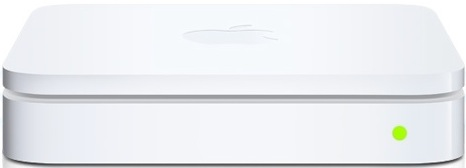
\includegraphics[width=3cm]{Figures/basestation.jpg} \\
{\tt WEP}, {\tt WPA/WPA2}
\end{center}
\end{minipage}
&
%\pause
\begin{minipage}{1.5cm}
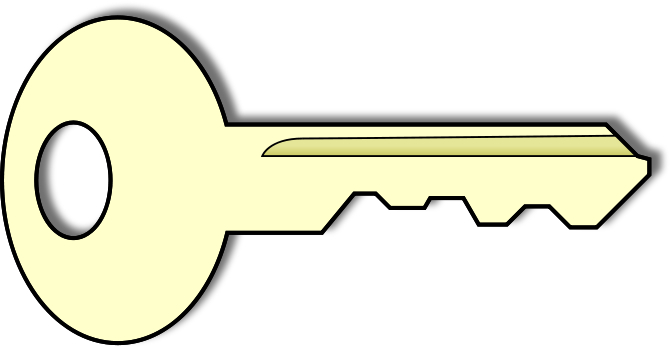
\includegraphics[width=1.5cm]{Figures/key.jpg} \\
{\tt SSL/SSH}
\end{minipage}
&
%\pause
\begin{minipage}{3cm}
\begin{center}
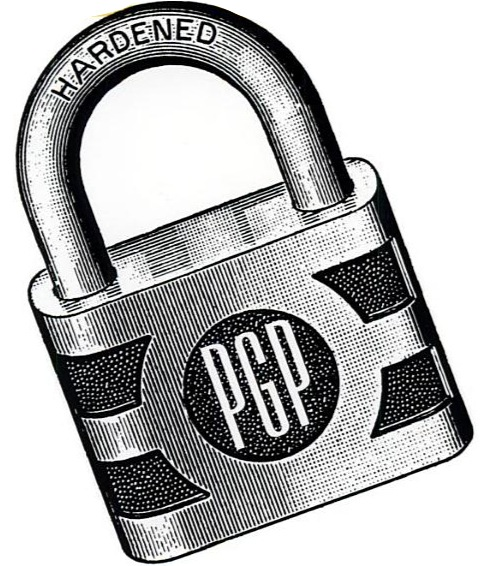
\includegraphics[width=2cm]{Figures/pgp.jpg} \\
{\tt PGP/GPG}
\end{center}
\end{minipage}
\\[1cm]
%\pause
\begin{minipage}{4cm}

\includegraphics[width=3cm]{Figures/amazon.jpg} \\
\begin{minipage}{4cm}
\tiny\tt
RSA Encryption
128 bytes: \\   
BE 89 0E A1 AD FA 7D 58 6A A1 6A E4 3B ED 75 E4 3E F2 19
F7 F3 0F FA D9 EF 62 10 52 7B FC DD 94 96 A8 35 6B 1B 50 60 2E 2E 79
AC 7C 2E A3 81 DE 8D 37 F9 EE 6E 4F 82 C7 E4 12 04 55 AF 57 69 94 8C
EF 2E 50 7A 6D 53 0F 5B 5F 62 58 5E CF F2 DF F4 4D CE 71 B6 82 D7 86
E5 4F 77 E4 91 AA E4 BD 5A 65 AA 9E 20 4F 38 5E B4 8B E0 36 45 80 A8
D5 24 5C 46 9D F1 80 C0 6B 62 A5 1F 26 5E AE 17 47
\end{minipage}
\end{minipage}
&
%\pause
\begin{minipage}{1.5cm}
\begin{center}

\includegraphics[width=1.3cm]{Figures/itunes.jpg} \\
DRM
FairPlay
\end{center}
\end{minipage}
&
%\pause
\begin{minipage}{3.5cm}
\begin{center}

\includegraphics[width=2.5cm]{Figures/mactexlogoX5.jpg} \\
{\tt MD5}
{\tiny\tt 5c3079df8a48623f5aa10f0181a7ab03}
\end{center}
\end{minipage}
\end{tabular}
\end{frame}

\begin{frame}
Cryptography is the art of \hl{computing} \&\ \hl{communicating} in
the presence of an \textcolor{red}{adversary}.
% Shafi Goldwasser, in the intro podcast to the MIT course

Cryptography is concerned with the conceptualization, definition, and
construction of computing systems that address security concerns.
% Oded Goldreich, in the intro to his Crypto book

% The following from pg 41 of "Network Security" by Kaufman, Perlman
% and Speciner
The word {\em cryptography} comes from the Greek word
$\kappa\rho\upsilon\pi\tau o$ (hidden or secret) and
$\gamma\rho\alpha\phi\eta$ (writing).  It can be seen as the art of
secret writing; this kind of crypto can provide services such as:
\begin{itemize}
\item  \df{integrity checking}: recipient is reassured that the
message was not altered;

\item  \df{authentication}: verifying someone's identity.
\end{itemize}
\end{frame}

\begin{frame}

But also $\ldots$

\begin{itemize}

\item  Download a package and check its {\tt MD5} signature; the
adversary here is the ``ether'' through which the package ``travels,''
e.g., {\em noisy channel}.

\item  Code ``obfuscation'' --- compile code so that it is executable
but cannot be reverse-engineered.

\item  Authentication: password login, client-server communication.

\item  Non-repudiation, electronic voting, digital cash, etc.
\end{itemize}
\end{frame}

\section{History}

\begin{frame}
\frametitle{Origins}

\begin{minipage}{3cm}
\raggedright
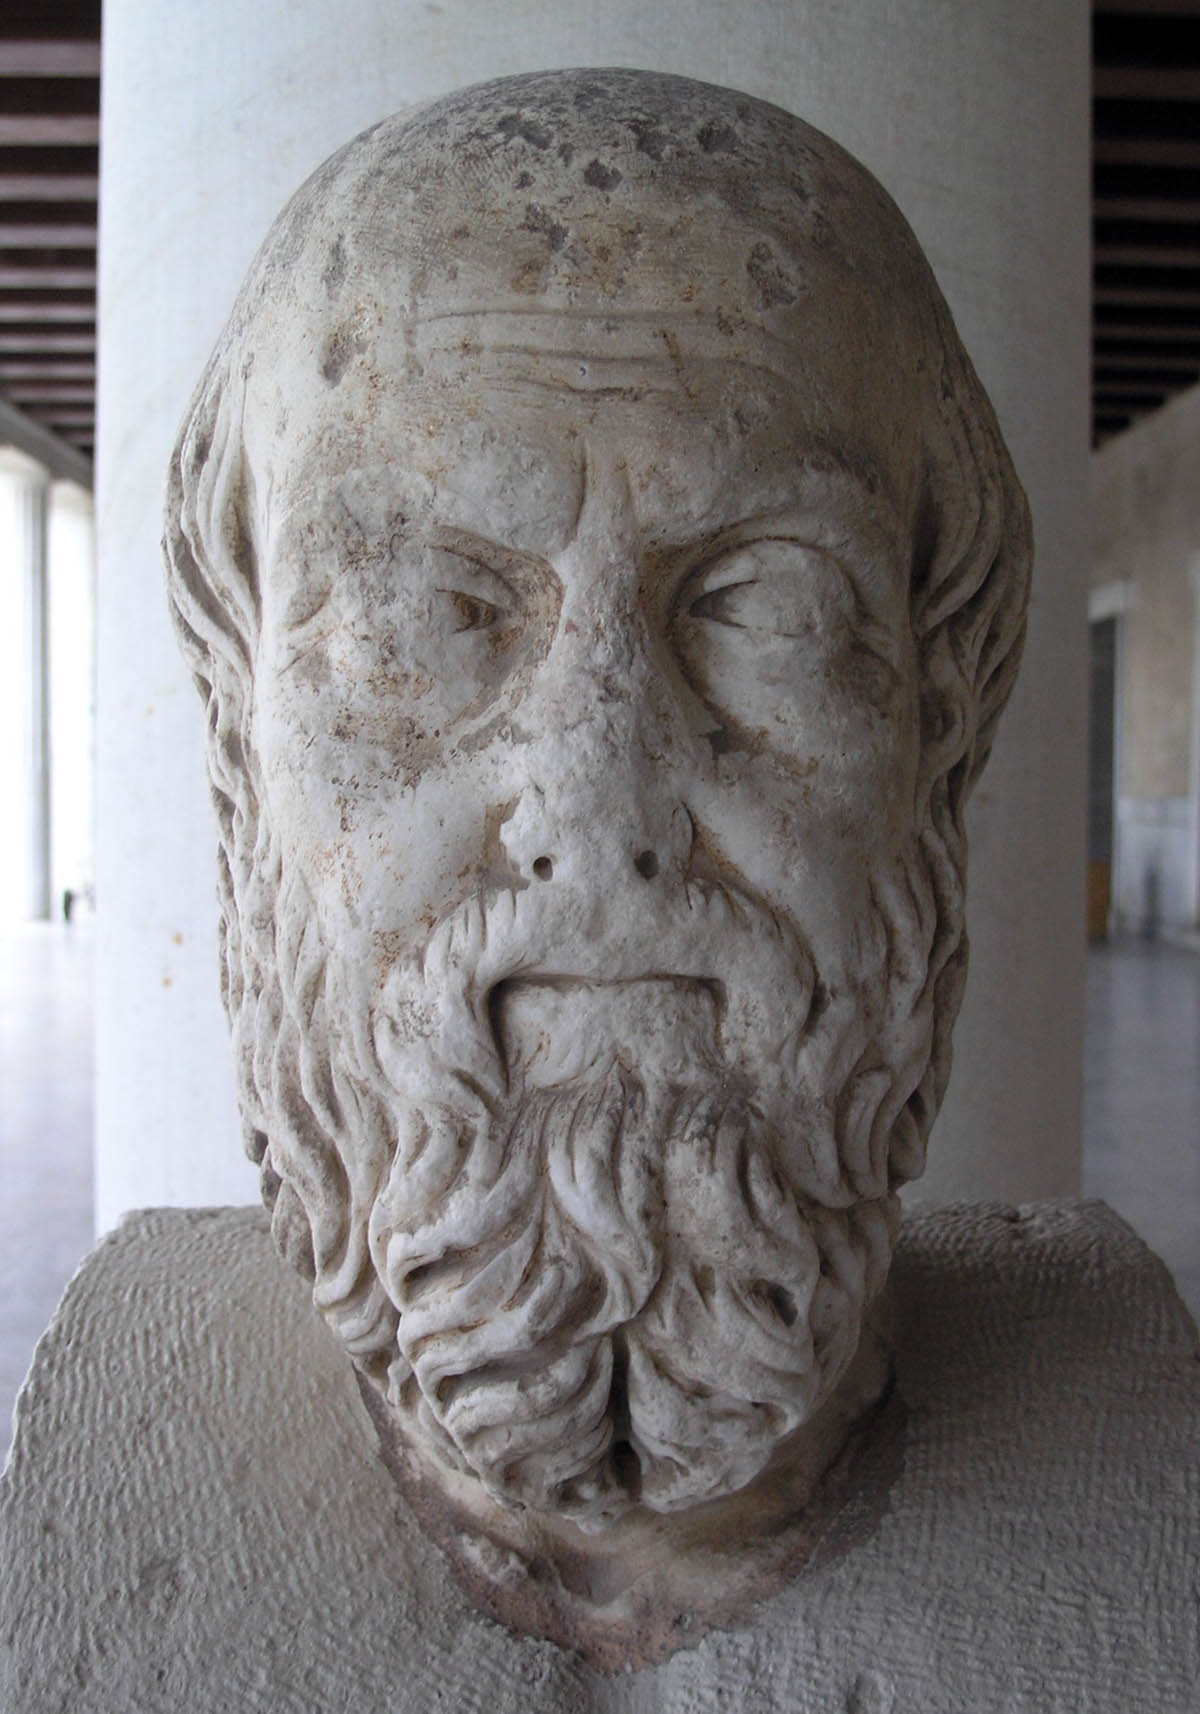
\includegraphics[width=2.6cm]{Figures/Herodotus.jpg} \\
\footnotesize
Herodotus chronicled the conflict between Greece \texttt{\&} Persia, 5BC.
\end{minipage}
\begin{minipage}{7cm}
\raggedright
\begin{itemize}
\item  Xerxes wanted to extend Persian empire; mobilizes a force.

\item  Persian military buildup witnessed by Demaratus.  Writes
message on wooden tablets, covers with wax and sends to Greece.

\item  Histaiaeus shaves the head of his messanger, writes the message
on the scalp, and waits for hair to grow back.

\item  \df{Steganography}
\end{itemize}
\end{minipage}
\end{frame}

\begin{frame}
\begin{center}
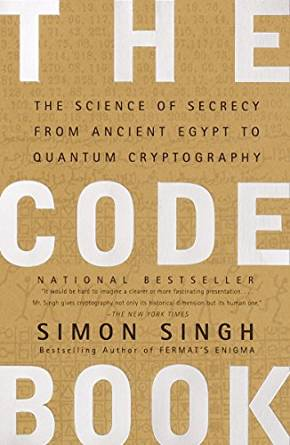
\includegraphics[width=4cm]{Figures/singh.jpeg} \\
Simon Singh, ``The Code Book.''
\end{center}
\end{frame}

\begin{frame}
\frametitle{Enigma machine}

\href{http://enigmaco.de/enigma/enigma.html}%
{\tt http://enigmaco.de/enigma/enigma.html}

\end{frame}

\begin{frame}
\begin{center}
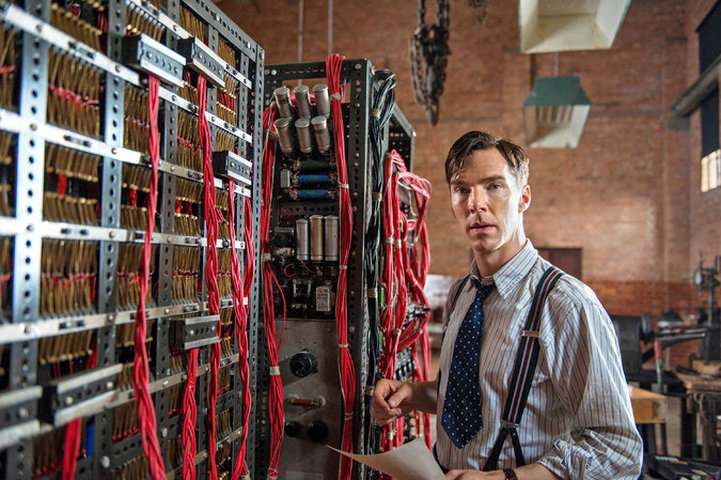
\includegraphics[height=4cm]{Figures/Imitation.jpg}
\hfill

\includegraphics[height=4cm]{Figures/Enigma.jpg} \\
Imitation Game (2014)\hfill Enigma (2001)
\end{center}
\end{frame}

\begin{frame}
\begin{center}
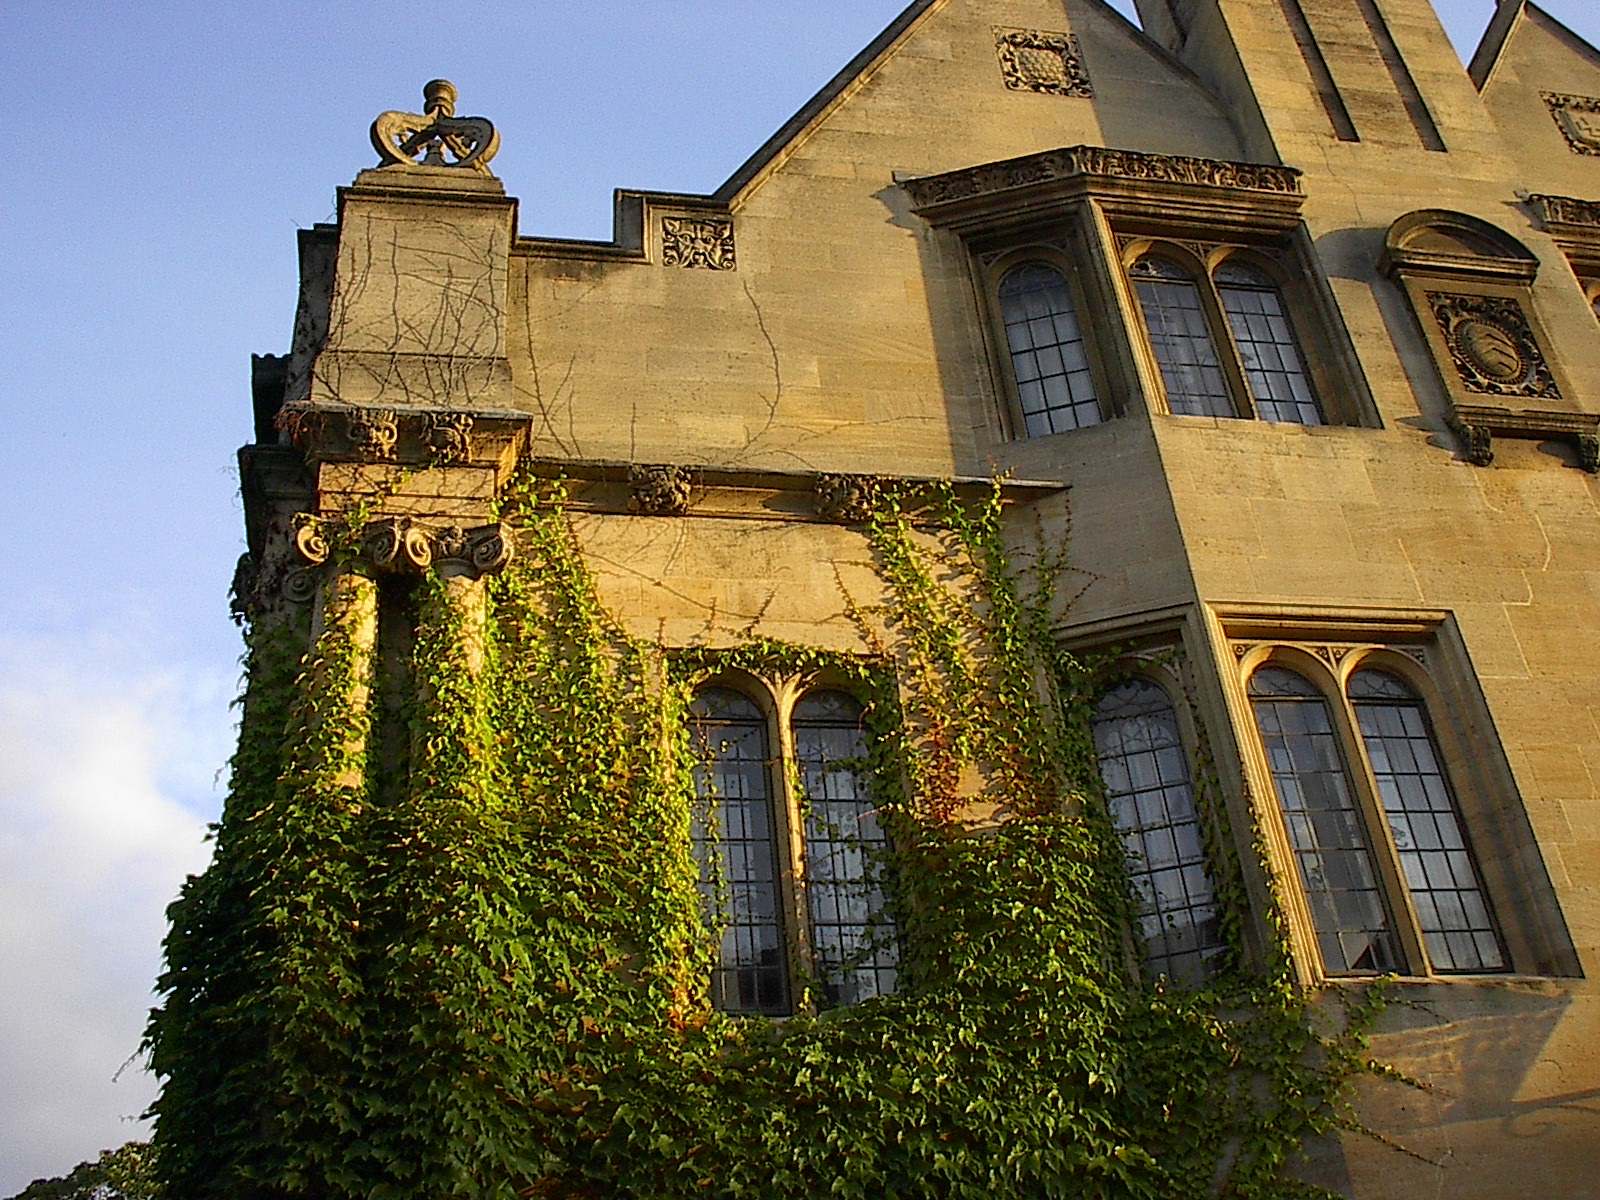
\includegraphics[width=3.5cm]{Figures/Oxford-1.jpg}
\hfill
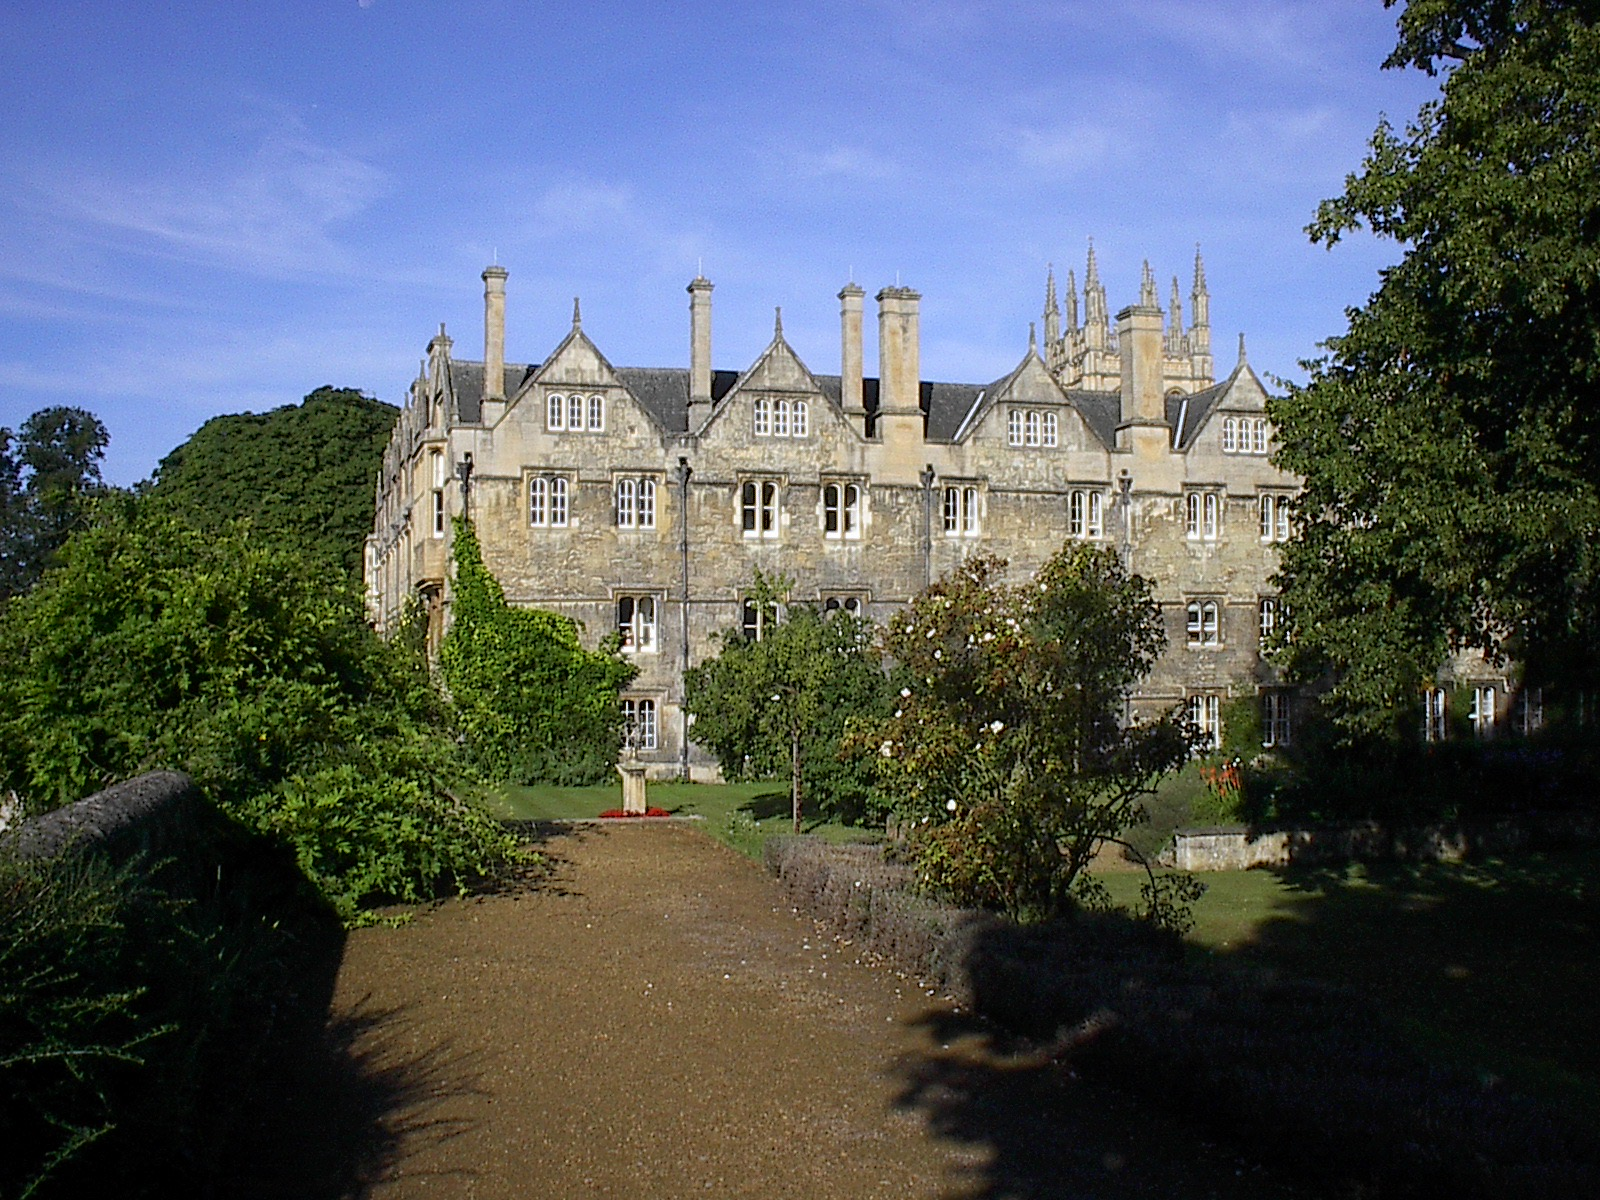
\includegraphics[width=3.5cm]{Figures/Oxford-2.jpg}
\hfill
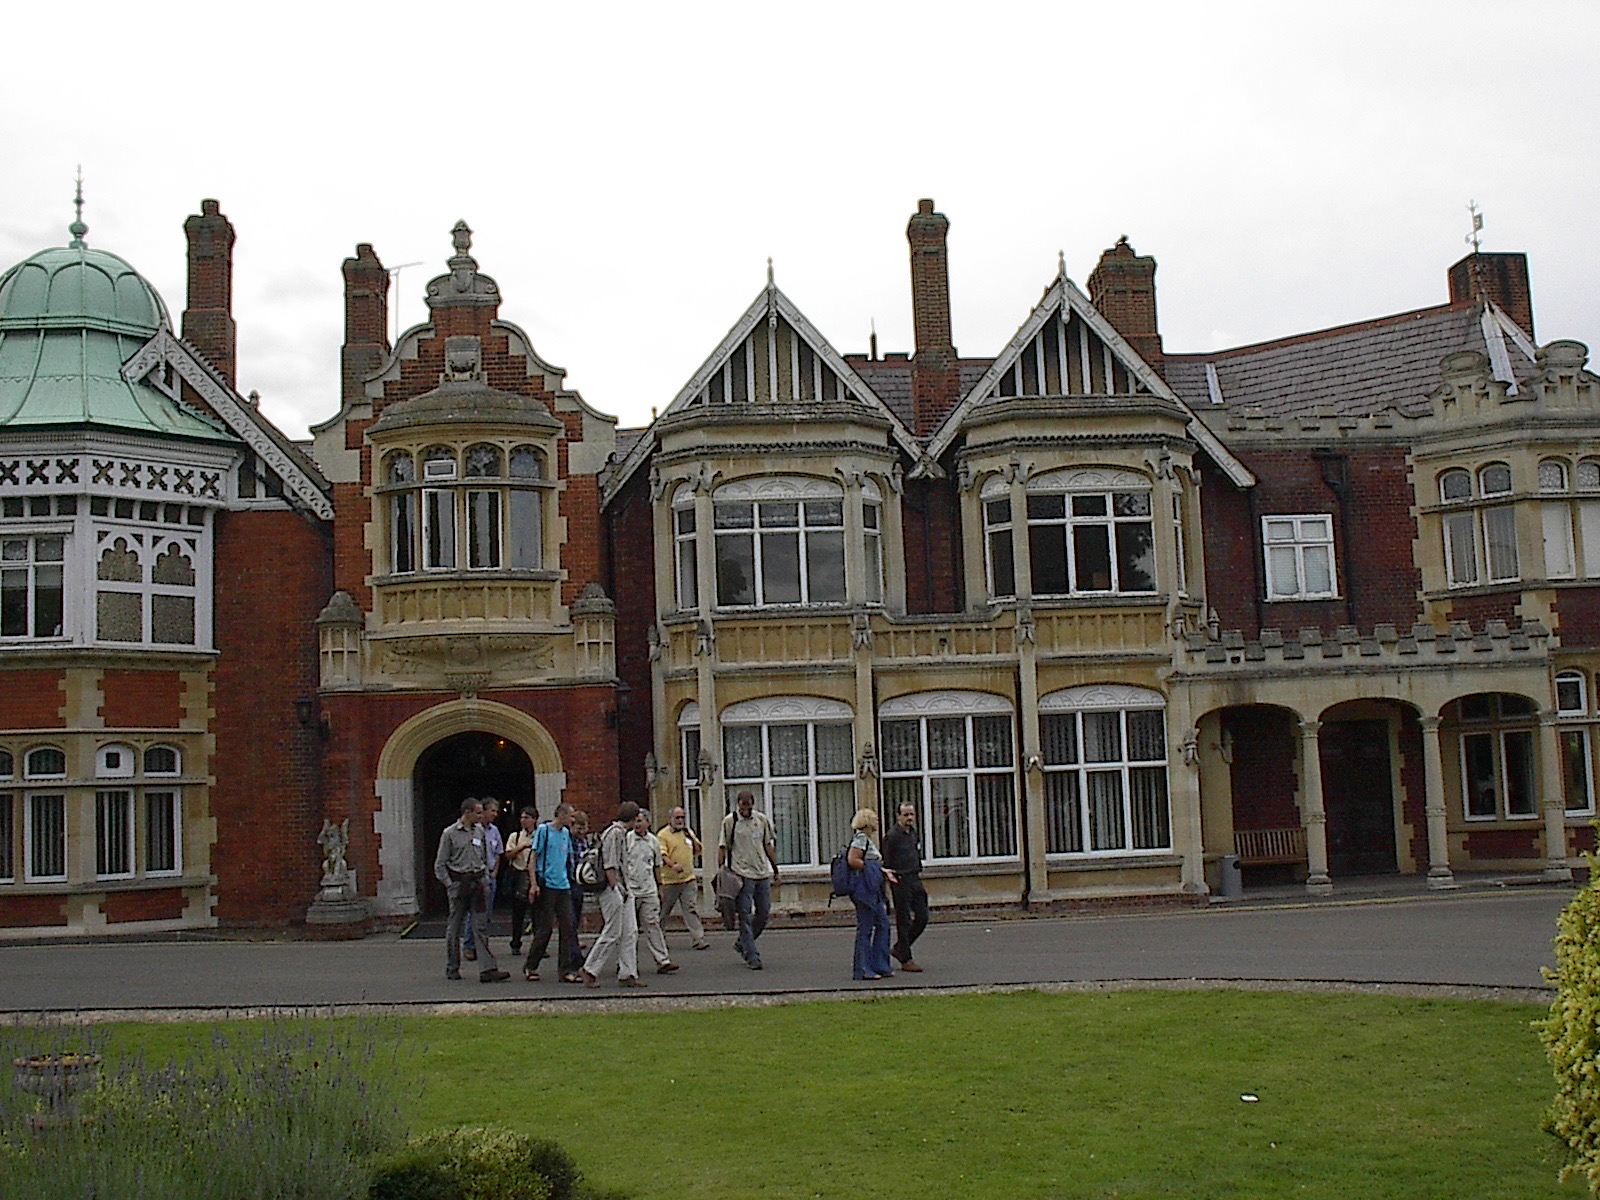
\includegraphics[width=3.5cm]{Figures/Bletchley.jpg} \\
Oxford (2005)\hfill Oxford (2005)\hfill Bletchley (2005)
\end{center}
\end{frame}

\begin{frame}
The \df{discrete logarithm problem (DLP)}

%\pause
Fix a group $G$ and $g\in G$: given an element $h\in\langle g\rangle$,
find an integer $m$ satisfying $h=g^m$.

%\pause
The smallest $m$ satisfying $h=g^m$ is the \df{logarithm} (or
\df{index}) of $h$ with respect to $g$ (written $m=\log_g(h)$).
\begin{center}
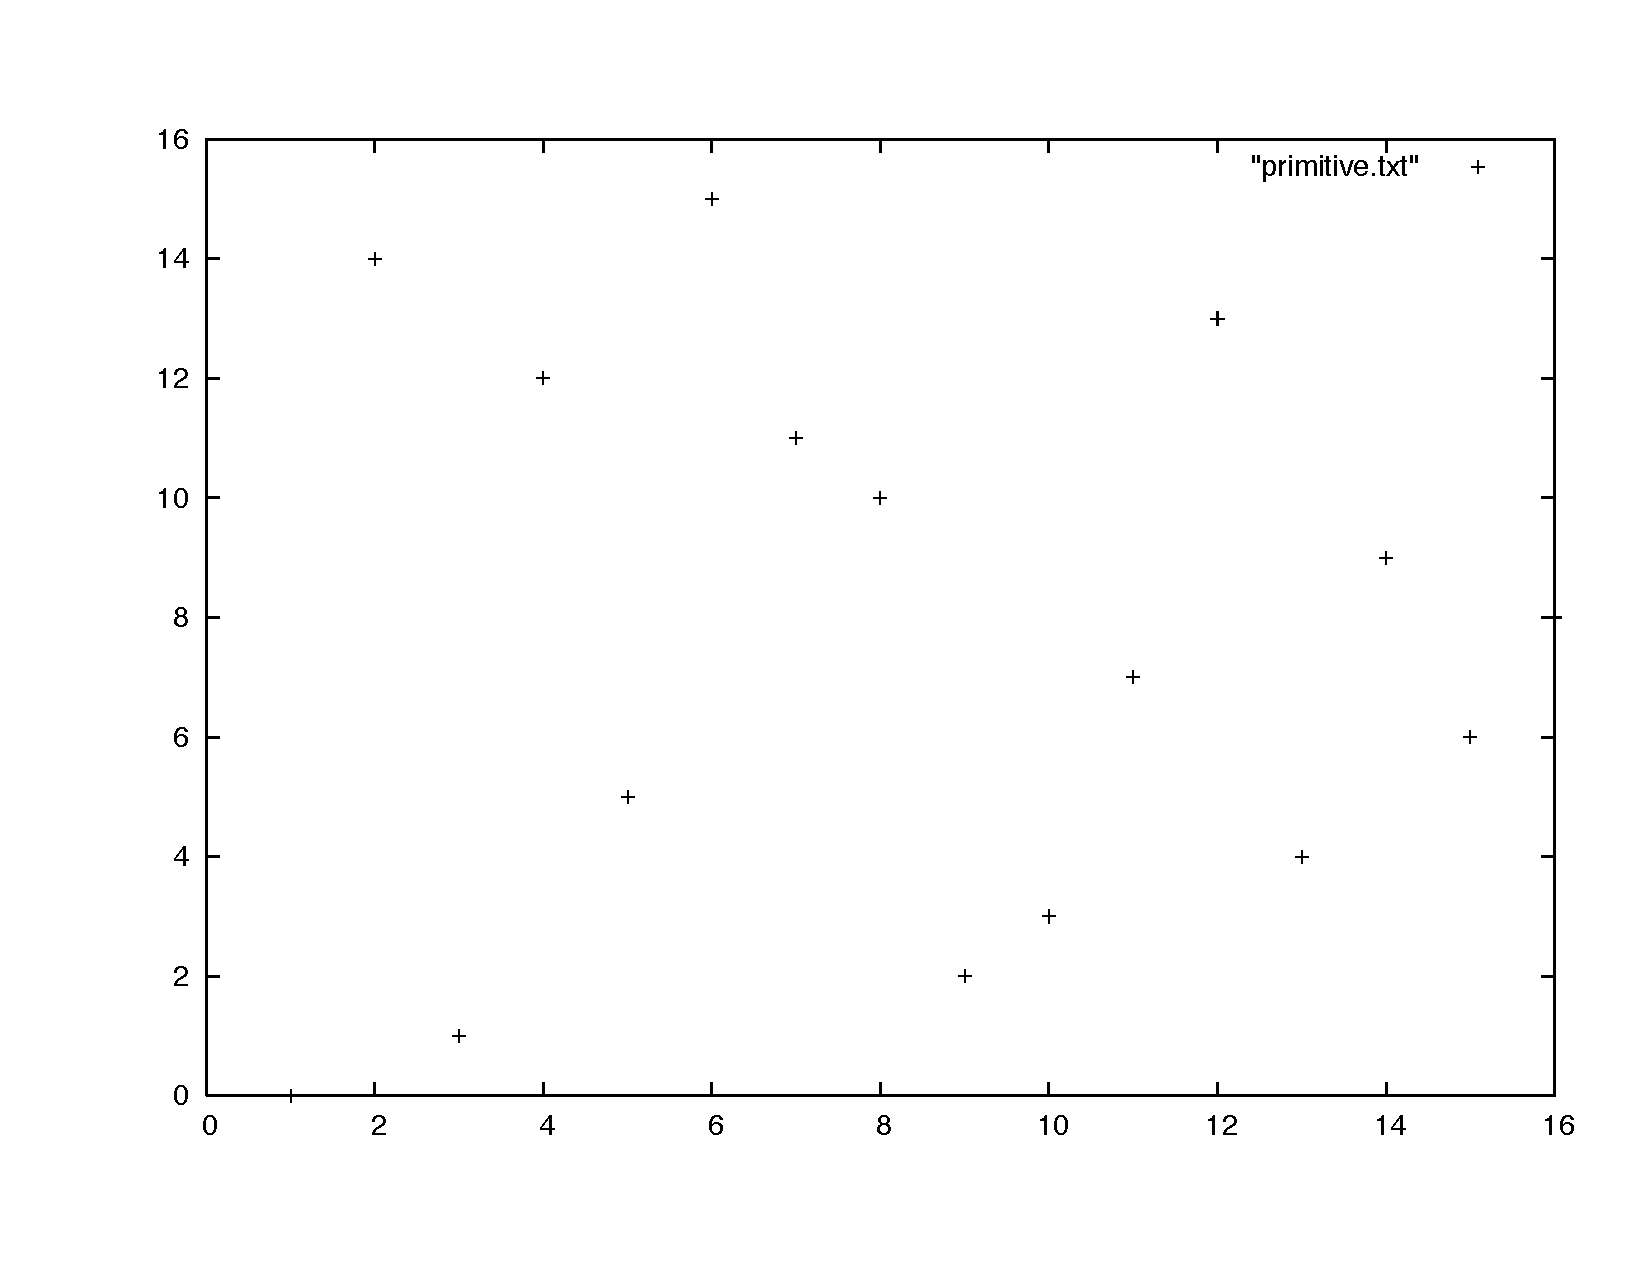
\includegraphics[width=6cm]{Figures/log.pdf}

Plot of $\log_3(x)$ over $\mathbb{Z}_{17}$.
\end{center}
\end{frame}

\begin{frame}
\frametitle{Shank's ``babystep-giantstep'' algorithm}

Computes $x$, such that $g^x\equiv_p h$,
in time $O(\sqrt{p}\log(\sqrt{p}))$.

\begin{algorithmic}[1] 
\REQUIRE $p$ prime, $\langle g\rangle=\mathbb{Z}_p^*$,
$h\in\mathbb{Z}_p^*$
   \STATE  $n\longleftarrow 1+\lfloor\sqrt{p}\rfloor$
   \STATE  $L_1\longleftarrow\{g^0,g^1,g^2,\ldots,g^n\}\pmod p$
   \STATE  $L_2\longleftarrow\{hg^0,hg^{-n},hg^{-2n},\ldots,hg^{-n^2}\}\pmod p$
   \STATE  Find $g^i\equiv_p hg^{-jn}\in L_1\cap L_2$
   \STATE  $x\longleftarrow jn+i$
   \RETURN $x$
\ENSURE $g^x\equiv_p h$
\end{algorithmic}
\end{frame}

\section{Public keys}

\begin{frame}
\frametitle{PKCs}

\begin{itemize}
\item Diffie-Hellman
\item ElGamal
\item RSA
\end{itemize}
\end{frame}

\subsection{Diffie-Hellman}

\begin{frame}
\frametitle{Diffie-Hellman Key Exchange}

\begin{itemize}
\item  Oldest public key cryptosystem still in use.
\item  Allows two individuals to \textcolor{blue}{agree on a shared
key}, even though they can \textcolor{blue}{only exchange messages in
public}.
\item  A weakness is that there is \textcolor{blue}{no
authentication}; the other might be a ``bad guy.''

\item  Described in {\tt RFC 2631} \\
\url{https://www.ietf.org/rfc/rfc2631.txt}
\end{itemize}
\end{frame}

\begin{frame}
\begin{tabular}{|lr|}\hline
Alice & Bob \\\hline
\multicolumn{2}{|c|}{\textcolor{blue}{Public: Group $G=\langle
g\rangle$ and $n=|G|=\text{ord}(g)$}} \\
Choose secret $0<a<n$             & Choose secret $0<b<n$ \\
Computer $A:=g^a$                 & Compute $B:=g^b$ \\
Send $A$ to Bob $\rightarrow$     & $\leftarrow$ Send $B$ to Alice \\
Compute $B^a$                     & Compute $A^b$ \\\hline
\multicolumn{2}{|c|}{Alice \&\ Bob have shared value} \\
\multicolumn{2}{|c|}{$A^b=(g^{a})^b=g^{ab}=g^{ba}=(g^b)^a=B^a$}
\\\hline
\end{tabular}
\end{frame}

\begin{frame}

\begin{enumerate}
\item  Alice and Bob agree to use a prime $p=23$ and base $g=5$.

\item  Alice chooses secret $a=8$; sends Bob $A=g^a \pmod p$
\begin{enumerate}
\item  $A = 5^8 \pmod{23}$
\item  \colorbox{yellow}{$A = 16$}
\end{enumerate}

\item  Bob chooses secret $b=15$; sends Alice $B = g^b \pmod p$
\begin{enumerate}
\item  $B = 5^{15} \pmod{23}$
\item  \colorbox{yellow}{$B = 19$}
\end{enumerate}

\item  Alice computes $s = B^a \pmod p$
\begin{enumerate}
\item  $s = 19^8 \pmod{23}$
\item  \colorbox{orange}{$s = 9$}
\end{enumerate}

\item Bob computes $s = A^b \pmod p$
\begin{enumerate}
\item  $s = 16^{15} \pmod{23}$
\item  \colorbox{orange}{$s = 9$}
\end{enumerate}
\end{enumerate}
\end{frame}

\begin{frame}
The Diffie-Hellman Problem (DHP): compute $g^{ab}$ from $g^a$ and
$g^b$.

%\pause
If we could solve the DLP easily, we could solve the DHP easily.

%\pause
For some groups DLP is easy: $(\mathbb{Z}_m,+)$, integers modulo $m$
under addition, or $(\mathbb{R}^+,\ast)$, positive reals under
multiplication.

%\pause
For some groups, such as $(\mathbb{Z}_m,\ast)$, integers modulo $m$
under multiplication, we believe that DLP is hard: the best known
algorithm takes time:
$$
O\left(e^{c\sqrt[3]{(\log m)(\log\log m)^2}}\right)
$$
\end{frame}

\begin{frame}
Diffie-Hellman enables two parties that have never communicated before to
establish a mutual secret key by exchanging messages over a public
channel.
DH only resists \df{passive adversaries}.

A \df{passive attack} is one in which the intruder eavesdrops but does
not modify the message stream in any way.

An \df{active attack} is one in which the intruder may:
\begin{itemize}
\item  transmit messages
\item  replay old messages
\item  modify messages in transit
\item  delete selected messages from the wire
\end{itemize}
A typical active attack is one in which an intruder impersonates one
end of the conversation, or acts as a \df{man-in-the-middle}.

How to do a ``man-in-the-middle'' on DH?
\end{frame}

\begin{frame}
In DH it is recommended to make prime $p$ 1024 bits long.

\df{DH assumption}: $k=g^{ab}$ hard to compute from $g^a$ and $g^b$ in
$\mathbb{Z}_p^*$.  

But, this does not guarantee that a particular bit
or group of bits of $k$ is also hard to compute.

Usually, the length of a symmetric session key is 128 bits.

Take the 128 most significant bits of $k=g^{ab}\pmod p$;
call this $\tilde{k}$.

$\tilde{k}$ is still hard to compute from $g^a$ and $g^b$.

In 1996 Boneh \&\ Venkatesan show that computing $\sqrt{|p|}$ most
significant bits is as hard as computing all the bits ($\sqrt{1024}=32$).
\end{frame}

\subsection{ElGamal}

\begin{frame}
\frametitle{ElGamal}

Alice and Bob agree on public $p,g$, such
that $p$ is a prime and $\mathbb{Z}_p^*=\langle g\rangle$.  

Alice also has a \hl{private $a$} and publishes a \hl{public
$A:=g^a\pmod p$}.

Bob wants
to send a message $m$ to Alice, so he creates an \df{ephemeral key
$b$}, and sends the pair $c_1,c_2$ to Alice where:
$$
c_1:=g^b\pmod p; \qquad c_2:=mA^b\pmod p.
$$
Then, in order to read the message, Alice computes:
$$
c_1^{-a}c_2\equiv_pg^{-ab}mg^{ab}\equiv_pm.
$$

\end{frame}

\begin{frame}

To compute $c_1^{-a}$ $A$ computes the inverse of
$c_1$ in $\mathbb{Z}_p^*$, using the
extended Euclid's algorithm (EEA), and
then compute the $a$-th power of the result. 

To compute the
inverse of some $k$ in $\mathbb{Z}_n^*$,
note first that
$\gcd(k,n)=1$.  

So using EEA we obtain ({\em feasibly}!)
$s,t$ such that $sk+tn=1$.
Then the inverse is $s\pmod n$.

\begin{algorithmic}[1]
\REQUIRE $m>0, n\ge 0$
\STATE $a\longleftarrow m$;
$b\longleftarrow n$
\IF{$b=0$}
        \RETURN $(a,1,0)$
\ELSE
        \STATE $(d,x,y)\longleftarrow\text{Euclid}(b,\rem(a,b))$
        \RETURN $(d,y,x-\text{div}(a,b)\cdot y)$
\ENDIF
\ENSURE $mx+ny=d=\gcd(m,n)$
\end{algorithmic}

%But $s$ is not necessarily in $\mathbb{Z}^*_n$; then we place it first
%in the set $\mathbb{Z}_n$ by adding an appropriate number of multiples
%of $n$, i.e., say $s+in\in\mathbb{Z}_n$ (where $i\in\mathbb{Z}$).
%Thus:
%$$
%(s+in)k+(t-ik)n = (sk+tk)+(ink-ikn) = (st+tk)+0 = 1 
%$$
%and this means also that $(s+in)k\equiv 1\pmod n$, and so
%$(s+in)\in\mathbb{Z}_n^*$ and it is the inverse of $k$.
\end{frame}

\subsection{Reductions}

\begin{frame}
\frametitle{Reductions}

We say that we can \df{break} ElGamal, if we have an efficient way for
computing $m$ from $\langle p,g,A,c_1,c_2\rangle$.  

{\bf Reductions:}
We can
break ElGamal if and only if we can solve the DHP efficiently.

The DHP on input $\langle p,g,A\equiv_p g^a,
B\equiv_p g^b\rangle$ outputs $g^{ab}\pmod p$, and the ElGamal problem,
call it ELGP, on input 
\begin{equation}\label{eq:elgpinput}
\langle p,g,A\equiv_p g^a, c_1\equiv_p g^b, c_2\equiv_p mA^b\rangle
\end{equation}
outputs $m$.  

We want to show that we can break Diffie-Hellman, i.e.,
solve DHP efficiently, if and only if we can break ElGamal, i.e.,
solve ELGP efficiently.  

The key-word here is \highlight{efficiently},
meaning in polynomial time.
\end{frame}

\begin{frame}
($\Rightarrow$)  Suppose we can solve DHP efficiently; we
give an efficient procedure for solving ELGP: given the
input~(\ref{eq:elgpinput}) to
ELGP, we obtain $g^{ab}\pmod p$ from 
$A\equiv_p g^a$ and $c_1\equiv g^b$
using the efficient solver for DHP.

We then use the extended Euclidean algorithm
to obtain $(g^{ab})^{-1}\pmod p$.
$$
c_2\cdot (g^{ab})^{-1}
\equiv_p mg^{ab}(g^{ab})^{-1}
\equiv_p m
=m
$$
where the last equality follows from $m\in\mathbb{Z}_p$.
\end{frame}

\begin{frame}
($\Leftarrow$) Suppose we have an efficient solver for the
ELGP.  To solve the DHP, we construct the following input to ELGP:
$$
\langle p,g,A\equiv_p g^a,c_1\equiv_p g^b,c_2=1\rangle.
$$
Note that $c_2=1\equiv_p\underbrace{(g^{ab})^{-1}}_{=m}A^b$, so using
the efficient solver for ELGP we obtain $m\equiv_p (g^{ab})^{-1}$, and
now using the extended Euclid's algorithm we obtain the inverse of
$(g^{ab})^{-1}\pmod p$, which is just $g^{ab}\pmod p$, so we output
that.
\end{frame}

\subsection{ElGamal signature scheme}

\begin{frame}
\frametitle{ElGamal signature scheme}

We sign the hash value of message.

$\mathbb{Z}_p^*=\langle g\rangle$ and $a$ is the secret key

\colorbox{yellow}{$k$ is random} and
$h:\mathbb{N}\longrightarrow\mathbb{Z}_p$ is a hash function

$1<g,a,k<p-1$, and $\gcd(k,p-1)=1$.

Compute:
\begin{align*}
r &:= g^k\pmod p \\
s &:= k^{-1}(h(m)-ar)\pmod{(p-1)}
\end{align*}

If $s$ is zero, start over again, by selecting a different $k$

The \highlight{signature of $m$} is the (ordered) pair of numbers $(r,s)$.  
\end{frame}

\begin{frame}

For example, with the following values:
$$
\begin{array}{llllll}
m = \texttt{A message.}
& h(m) = 5
& p = 11
& g = 6
& a = 3
& k = 7
\end{array}
$$
the signature of `A message.' will be:
\begin{align*}
r &= 6^7\pmod{11}=8 \\
s &= 7^{-1}(5-3\cdot 8)\pmod{(11-1)} \\
  &= 3\cdot(-19)\pmod{10}=3\cdot 1\pmod{10}=3
\end{align*}
i.e., $\text{sign}(\text{A message.})=(8,3)$.
\end{frame}

\begin{frame}

Suppose $h(m)$ is obtained by multiplying the ASCII values of the
symbols in the message modulo $11$.

Messages ``A mess'' and ``L message'' have the same hash value.  

In general, by its nature, any
hash function is going to have such \df{collisions}, i.e., messages
such that:
$$
h(\text{A message.})=h(\text{A mess})=h(\text{L message})=5,
$$
but there are hash functions which are \df{collision-resistant} in
the sense that it is computationally hard to find two messages $m,m'$
such that $h(m)=h(m')$.  

A good hash function is also a \df{one-way
function} in the sense that given a value $y$ it is computationally
hard to find an $m$ such that $h(m)=y$.

\end{frame}

\begin{frame}

If you receive a message $m$, and a signature pair $(r,s)$, and
you only know $p,g$ and $A=g^a\pmod p$, i.e., $p,g,A$ are the {\em
public} information, how can you ``verify'' the signature---and what
does it mean to verify the signature?

Verifying the signature means checking that it was
the person in possession of $a$ that signed the document $m$.  

Two
subtle things: first we say ``in possession of $a$'' rather than the
``legitimate owner of $a$,'' simply because $a$ may have been
compromised (e.g., stolen).  This is not an {\em authentication}
scheme!  

Second, and this is why this scheme
is so brilliant, we can check that ``someone in possession of $a$''
signed the message, even {\em without knowing what $a$ is}!  

We know
$A$, where $A=g^a\pmod p$, but for large $p$, it is difficult to
compute $a$ from $A$ (DLP).
\end{frame}

\begin{frame}
Here is how we verify that ``someone in possession of $a$'' signed the
message $m\in\mathbb{N}$.  

First we check $0<r<p$ and $0<s<p-1$. 

Then we compute
\begin{align*}
v &:= g^{h(m)}\pmod p\\
w &:= A^rr^s\pmod p
\end{align*}
Remember that $g,p$ are public, $m$ is
known, and the function $h:\mathbb{N}\longrightarrow[p-1]$ is also
known, and $r,s$ is the given signature.  

If $v=w$ then
the signature is valid.
\end{frame}

\begin{frame}
To see that this works note that we defined
\begin{align*}
s &:= k^{-1}(h(m)-ar)\pmod{p-1} \\
  &\Rightarrow h(m)\equiv ar+sk\pmod{p-1}\tag*{\text{$(\ast)$}}
\end{align*}
Fermat's Little Theorem says
that $g^{p-1}\equiv 1\pmod p$, and therefore
$$
g^{h(m)}\stackrel{(\ast\ast)}{\equiv}g^{ar+sh}
\equiv (g^a)^r(g^k)^s
\equiv A^rr^s\pmod p.
$$
The FLT is applied in the $(\ast\ast)$ equality:  from~($\ast$)
it follows that $(p-1)|(h(m)-(ar+sk))$, which
means that $(p-1)z=h(m)-(ar+sk)$ for some $z$, and since
$g^{(p-1)z}=(g^{(p-1)})^z=1^z=1\pmod p$, it follows that
$g^{h(m)-(ar+sk)}=1\pmod p$, and so $g^{h(m)}=g^{ar+sk}\pmod p$.

\end{frame}

\begin{frame}

%% The following questions (and their answers) can be found in Delfs &
%% Knebl, "Intro to Crypto", on page 73.

Without a ({\em good}) hash function, ElGamal's signature scheme is
\df{existentially forgeable}; i.e., an adversary Eve can construct a
message $m$ and a valid signature $(r,s)$ for $m$.

To see this, let $b,c$ be numbers s.t.\
$\gcd(c,p-1)=1$, and set  
\begin{align*}
r &:= g^bA^c \\ 
s &:= -rc^{-1}\pmod{p-1} \\
m &:= -rbc^{-1}\pmod{p-1}
\end{align*}
Then $(m,r,s)$ satisfies $g^m=A^rr^s$.

Since in practice a hash function $h$ is applied to the message, and
it is the hash value that is signed, to forge a signature for a
meaningful message is not easy:  

An adversary has to find a meaningful message \highlight{$m$} such that
$h(\text{\highlight{$m$}})\equiv -rbc^{-1}\pmod{p-1}$, which is hard.
\end{frame}

\begin{frame}
In practice $k$ is a random number;
it is absolutely necessary to choose a {\em new} random number for
each message.

If the same random number $k$ is used in two
different messages $m\neq m'$, then it is possible to compute $k$
as follows: 

$s-s'=(h(m)-h(m'))k^{-1}\pmod{p-1}$, and hence
$$
k=(s-s')^{-1}(h(m)-h(m'))\pmod{p-1}
$$

Once we have $k$, we can compute $a$.

\end{frame}

\begin{frame}
In the verification
it is essential to check that $1\le r\le p-1$. 

Otherwise $E$ would be able to sign a message of his choice, provided
he knows one valid signature $(r,s)$ for some message $m$, where $m$
is such that $1\le m\le p-1$ and $\gcd(m,p-1)=1$.

\begin{minipage}{5cm}
\raggedright
Let $m'$ be a message of $E$'s choice,
\begin{align*}
u  &\equiv m'm^{-1}\pmod{p-1} \\
s' &\equiv su\pmod{p-1}
\end{align*}
\end{minipage}
\vline\hskip 3mm
\begin{minipage}{5cm}
\raggedright
Let $r'$ be any integer such that
\begin{align*}
r' &\equiv r\pmod p \\
r' &\equiv ru\pmod{p-1}
\end{align*}
such an $r'$ can be obtained by Chinese Reminder Theorem.  
\end{minipage}

{\bf Exercise:} Show $(m',r',s')$ passes the verification.
\end{frame}

\subsection{RSA}

\begin{frame}
\frametitle{RSA\footnote{Rivest-Shamir-Adleman}}

\begin{itemize}
\item  The most commonly used key length for RSA is 1024 bits.
\item  The plaintext block must be smaller than the key.
\item  The ciphertext block will be the length of the key.
\item  RSA is \textcolor{blue}{much slower} than secret key algorithms
such as DES and IDEA.
\item  It is mostly used to secuerly exchange a secret key which is
then used for symmetric key encryption.
\item  Security: to factor a 512-bit number takes, with today's
technology, 30 thousand MIPS-years.
\item  {\tt RFC 2437}
\end{itemize}

\end{frame}

\begin{frame}
Choose two odd primes $p,q$, and set $n=pq$.  

Choose $k\in\mathbb{Z}^*_{\phi(n)}$, $k>1$.  

Advertise $f$, where $f(m)\equiv m^k\pmod n$.  

Compute $l$, the inverse of $k$ in $\mathbb{Z}^*_{\phi(n)}$.

Now $\langle n,k\rangle$ are public, and the key $l$ is secret, and so
is the function $g$, where $g(C)\equiv C^l\pmod n$.  

Note that $g(f(m))\equiv_n m^{kl}\equiv_n m$.
\end{frame}

\begin{frame}
Why $m^{kl}\equiv_n m$?  

Observe that
$kl=1+(-t)\phi(n)$, where $(-t)>0$,
and so $m^{kl}\equiv_n m^{1+(-t)\phi(n)}\equiv_n m\cdot
(m^{\phi(n)})^{(-t)}\equiv_n m$, because $m^{\phi(n)}\equiv_n 1$.

Note that this last statement does not follow
directly from Euler's theorem
because $m\in\mathbb{Z}_n$, and not
necessarily in $\mathbb{Z}^*_n$.

To make sure that $m\in\mathbb{Z}^*_n$ it is enough to insist that
we have $0<m<\min\{p,q\}$; so we
break a large message into small pieces.  
\end{frame}

\begin{frame}
It is interesting to note that we can bypass Euler's theorem, and
just use
Fermat's Little
theorem: 

We know that $m^{(p-1)}\equiv_p 1$ and $m^{(q-1)}\equiv_q 1$,
so $m^{(p-1)(q-1)}\equiv_p 1$ and $m^{(q-1)(p-1)}\equiv_q 1$, thus
$m^{\phi(n)}\equiv_p 1$ and $m^{\phi(n)}\equiv_q 1$.  

This means that
$p|(m^{\phi(n)}-1)$ and $q|(m^{\phi(n)}-1)$, so, since $p,q$ are
distinct primes, it follows that $(pq)|(m^{\phi(n)}-1)$, and so
$m^{\phi(n)}\equiv_n 1$.
\end{frame}

\begin{frame}
Clifford Cocks, a British mathematician working for the UK
intelligence agency GCHQ, described an equivalent system in an
internal document in 1973, but given the relatively expensive
computers needed to implement it at the time, it was mostly considered
a curiosity and, as far as is publicly known, was never deployed. 

His discovery, however, was not revealed until 1997 due to its
top-secret classification, and Rivest, Shamir, and Adleman devised RSA
independently of Cocks's work.
\end{frame}

\end{document}
